\documentclass[11pt]{article}
\usepackage[a4paper,margin=1.9cm]{geometry}
\usepackage{graphicx}
\usepackage{booktabs}
\usepackage{amsmath}
\usepackage[hidelinks]{hyperref}
\usepackage{titlesec}
\usepackage{caption}
\usepackage{float}
\usepackage{array}

\captionsetup{font=small,labelfont=bf}
\titlespacing*{\section}{0pt}{1.5ex}{0.5ex}
\titleformat{\section}{\large\bfseries}{}{0em}{}
\setlength{\parskip}{0.4em}
\setlength{\parindent}{0pt}
\newcommand{\code}[1]{\texttt{\small #1}}

\begin{document}

\begin{center}
{\LARGE\bfseries The Alpha Factory}\\[3pt]
{\normalsize A strategy factory and a four-layer validation gate \;$\cdot$\; Clarion Capital take-home}\\[3pt]
{\footnotesize Pre-registered criteria SHA-256 \code{8e35cb{\ldots}d5d8eab} \;$\cdot$\; full technical report in \code{report/report.pdf}}
\end{center}

\vspace{2pt}
\hrule height 0.7pt
\vspace{8pt}

{\bfseries Verdict: 48 candidates in, 0 survivors out.}\enspace A factory builds 48 strategies
from two opposed market hypotheses; a four-layer gate, run independently on all of them, lets
none through. The strongest, an ETH trend at 1.17 net Sharpe, fails on two counts: it breaches
the drawdown cap in the 2020 crash, and its Deflated Sharpe is 0.35 against a 0.95 bar. The
deliverable is the machine and the honest result, not an alpha.

\vspace{6pt}
\begin{center}\small
\renewcommand{\arraystretch}{1.15}
\begin{tabular}{@{}cccccc@{}}
\toprule
Strategies & Opposed families & Markets & Survivors & Best net Sharpe & Best Deflated Sharpe \\
\midrule
48 & 2 & 4 & 0 & 1.17 & 0.35 \;(0.95 to pass) \\
\bottomrule
\end{tabular}
\end{center}
\vspace{2pt}

\begin{figure}[H]\centering
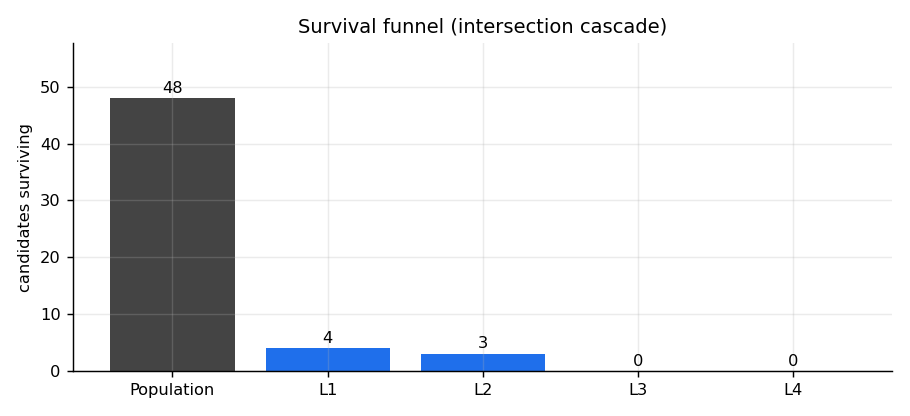
\includegraphics[width=0.60\linewidth]{figures/funnel.png}
\caption{The survival funnel: 48 candidates enter, 0 pass all four independent layers.}
\end{figure}

\textbf{The factory.} 48 instances = 2 opposed families $\times$ 6 parameter settings $\times$ 4
markets (S\&P 500, USD/JPY, gold, ETH), each with at most two free parameters. Being opposed by
construction, their signals are negatively correlated ($\approx-0.30$) and their returns nearly
uncorrelated across families: genuine diversification, not one bet in disguise.

\begin{center}\small
\renewcommand{\arraystretch}{1.25}
\begin{tabular}{@{}>{\bfseries}l l l@{}}
\toprule
Family & The bet & Free parameters \\
\midrule
voltarget\_mom & Trend: ride the move, sized to constant vol (cap $2\times$) & lookback, vol window \\
bollinger\_revert & Reversal: fade extremes, only in calm regimes & lookback, $z$-threshold \\
\bottomrule
\end{tabular}
\end{center}

\section{How the gate works}
Four independent, pre-registered tests run on the full population; survivors are their
\emph{intersection}, not a sequential filter, which is what exposes that L4 alone rejects all 48.

\begin{center}\small
\renewcommand{\arraystretch}{1.2}
\begin{tabular}{@{}l l c l@{}}
\toprule
\textbf{Layer} & \textbf{What it tests} & \textbf{Pass} & \textbf{Dominant failure} \\
\midrule
L1 & Out-of-sample edge $+$ $\pm20\%$ robustness & 4 / 48 & OoS Sharpe below bar \\
L2 & Walk-forward stability across windows & 6 / 48 & out-of-window Sharpe/return low \\
L3 & Stress: COVID $+$ own worst windows $+$ $2\times$ vol & 8 / 48 & blows up in the COVID window \\
L4 & Block-permutation significance $+$ Deflated Sharpe & 0 / 48 & fails the Deflated Sharpe \\
\midrule
\multicolumn{2}{@{}l}{\textbf{Survivors $=$ intersection of all four}} & \textbf{0 / 48} & \\
\bottomrule
\end{tabular}
\end{center}

\section{Why nothing survives}
The binding constraint is the \textbf{Deflated Sharpe}, which corrects a Sharpe for the number of
strategies tried. The luckiest of 48 zero-skill trials would be expected to score $\approx1.32$
annualised; the best candidate's 1.17 sits \emph{below} that luck hurdle, for a Deflated Sharpe of
just 0.35. Crediting the correlation among trials (an effective $\approx12$ rather than 48) lifts
it only to 0.69, still short of 0.95. Generating \emph{more} candidates cannot manufacture a
survivor, because each one raises the bar for all of them.

\begin{figure}[H]\centering
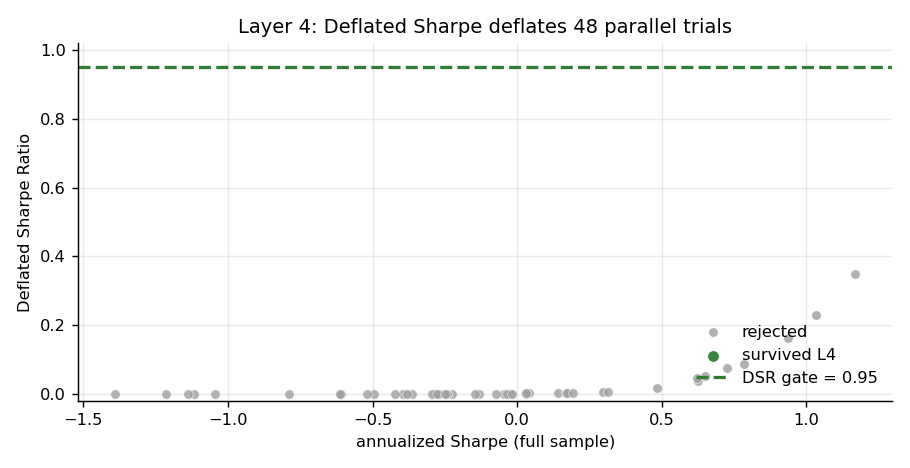
\includegraphics[width=0.60\linewidth]{figures/dsr_scatter.png}
\caption{Deflated Sharpe vs.\ net Sharpe across the 48. None clears 0.95; the best reaches 0.35.}
\end{figure}

\section{Where the costs bite}
The two families fail for different reasons: reversion is low-turnover but weak \emph{even gross},
so costs are not what kill it; trend is high-turnover (it re-scales every bar to hold volatility
constant) and is where costs bite, the median trend instance falling from a gross Sharpe of 0.59
to 0.11 net.

\begin{figure}[H]\centering
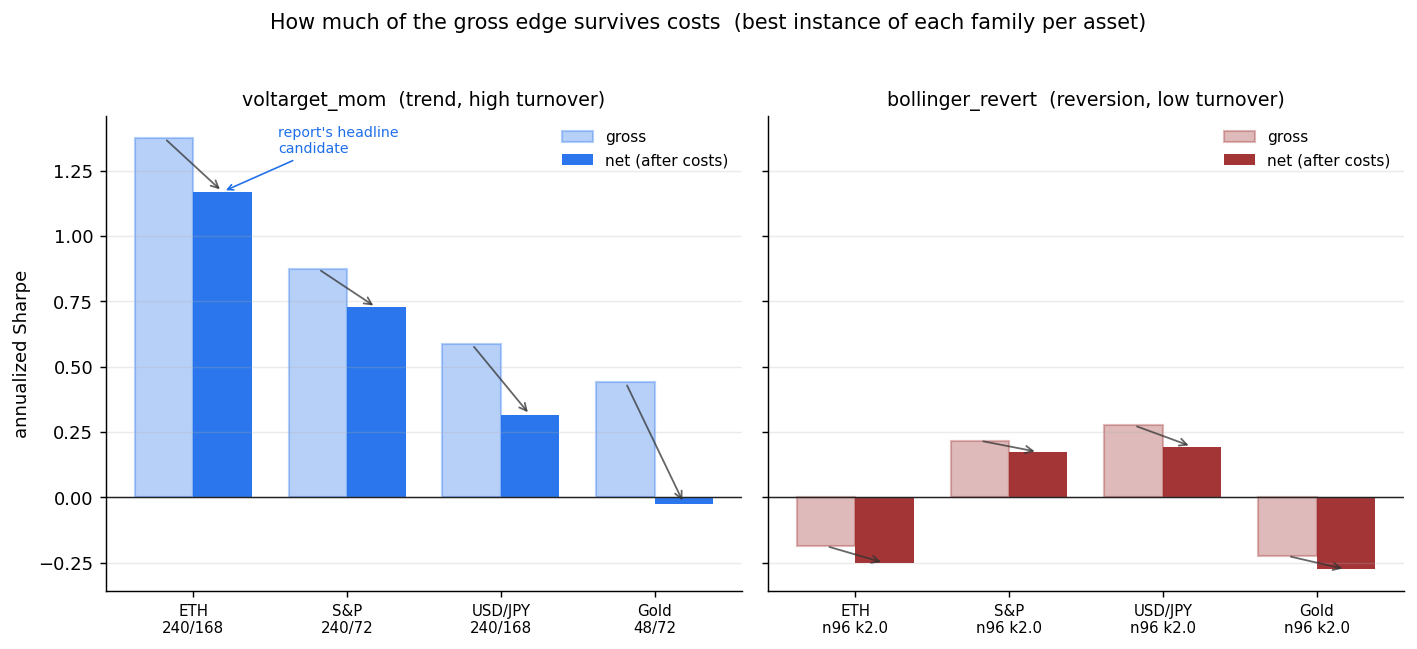
\includegraphics[width=0.74\linewidth]{figures/cost_drag.png}
\caption{Gross vs.\ net Sharpe, best instance per market. Costs barely touch the low-turnover
reversion grid but materially erode the high-turnover trend grid.}
\end{figure}

\section{Honesty, reproducibility, and what comes next}
Every threshold was fixed in \code{config/gate\_criteria.yaml} and SHA-256-hashed \emph{before}
the gate ran; the hash held across every strategy iteration (one documented L2 redesign aside),
so no bar was ever tuned to admit a winner. The pipeline is deterministic and reproduces
$48\to0$ from the raw data with \code{python run.py}. And the path forward is \emph{not} a richer
factory, since more variations only raise the deflation bar: it is more history, genuinely
orthogonal alpha (new data or a different economic rationale), and combining several weak but
uncorrelated signals at the portfolio level. Better ideas and more data, never a looser gate.

\end{document}
